\recipe{Vegetarian Thai Green Curry}
\label{recipe:veggie_thai_green_curry}
\makes{4 portions}
\worktime{\SI{30} \minute}
\totaltime{\SI{30} \minute}
\source{Murray}


\begin{ingredients}

  \item 2 tbsp vegetable oil
  \item 3 shallots - finely sliced
  \item 4 tbsp Thai green curry paste
  \item 1 red chilli - deseeded and finely chopped
  \item 350g butternut squash - peeled and cut into 1.5cm cubes
  \item 1 large red pepper - deseeded and cut into thick slices
  \item 400g can full fat coconut milk
  \item 5 lime leaves
  \item 150g mangetout
  \item 100g baby corn - halved lengthways
  \item 1 small bunch coriander  roughly chopped
  \item cooked rice
  \item lime wedges
\end{ingredients}


\begin{method}
  	Heat the oil in a large flameproof casserole dish with a tight-fitting lid.
Add the shallots with a generous pinch of salt and fry for 7-10 mins
over a medium heat until softened and beginning to caramelise. Add
the curry paste and chilli to the dish and fry for 2 mins. Tip in the
squash and pepper, then stir through the coconut milk along with
200ml water. Add the lime leaves, cover and cook for 15-20 mins or
until the squash is tender.

Stir the mangetout and baby corn through the curry, then re-cover,
cooking over a medium-low heat for a further 5 mins or until the veg
is just cooked. Season and stir through half the coriander. Remove the
lime leaves and discard. Spoon the curry into deep bowls, scatter with
the remaining coriander and serve with rice and lime wedges for
squeezing over.
  
\end{method}


\begin{figure}[h]
  	\centering
  	
  	\begin{tikzpicture}
  		% Save the image in a box to get its dimensions
  		\sbox0{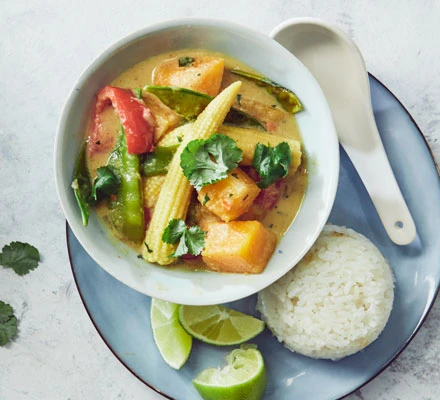
\includegraphics[width = 0.6\linewidth]{images/veg_thai_curry.png}}%
  
  		% Draw a clipping rectangle with rounded corners
  		\path[clip, rounded corners=0.5cm] (0,0) rectangle (\wd0,\ht0);
  
  		% Place the image inside the clipped area
  		\node[inner sep=0pt, outer sep=0pt, anchor=south west] at (0,0) {\usebox0};
	\end{tikzpicture}

\end{figure}


